\documentclass[11pt,a4paper]{article}

\usepackage[margin=1.05in]{geometry}
\usepackage{amsmath,amssymb,amsthm}
\usepackage{graphicx}
\usepackage{mathtools}
\usepackage{stmaryrd}
\usepackage{booktabs}
\usepackage{xcolor}
\usepackage{tikz}
\usetikzlibrary{arrows.meta,positioning,calc}
\usepackage[colorlinks=true,linkcolor=black,citecolor=black,urlcolor=blue]{hyperref}
\usepackage{enumitem}
\usepackage[protrusion=true,expansion=false]{microtype}
\setlength{\emergencystretch}{2.5em}

%%%%%%%%%%%%%%%%%%%%%%%%%%%%%%%%%%%%%%%%%%%%%%%%%%%%%%%%%%%%%%%%%%%%%%%%%%%%%%%
\theoremstyle{plain}
\newtheorem{theorem}{Theorem}[section]
\newtheorem{proposition}[theorem]{Proposition}
\newtheorem{lemma}[theorem]{Lemma}
\newtheorem{corollary}[theorem]{Corollary}
\theoremstyle{definition}
\newtheorem{definition}[theorem]{Definition}
\newtheorem{example}[theorem]{Example}
\newtheorem{finding}[theorem]{Empirical finding}
\theoremstyle{remark}
\newtheorem{remark}[theorem]{Remark}

%%%%%%%%%%%%%%%%%%%%%%%%%%%%%%%%%%%%%%%%%%%%%%%%%%%%%%%%%%%%%%%%%%%%%%%%%%%%%%%
% NOTATION RULES: the rho calculus is never written with the Greek letter;
% quoting is @P, dropping is *x.
%%%%%%%%%%%%%%%%%%%%%%%%%%%%%%%%%%%%%%%%%%%%%%%%%%%%%%%%%%%%%%%%%%%%%%%%%%%%%%%
\let\oldsc\textsc
\renewcommand{\textsc}[1]{\textup{\oldsc{#1}}}
\newcommand{\rhoc}{\textsf{rho}}
\newcommand{\V}{\mathbb{V}}
\newcommand{\Rnn}{\mathbb{R}_{\geq 0}}
\newcommand{\Qp}{\mathbb{Q}_{>0}}
\newcommand{\Cx}{\mathbb{C}}
\newcommand{\scong}{\equiv}
\newcommand{\nameq}{=_{\mathsf{N}}}
\newcommand{\tensorv}{\otimes}
\newcommand{\sumv}{\oplus}
\newcommand{\crisp}[1]{\lceil #1 \rceil}
\newcommand{\Pit}{\Pi}
\newcommand{\Dur}{\Delta}
\newcommand{\Tim}{\mathcal{T}}
\newcommand{\nm}[3]{\langle @#1,\,#2,\,#3\rangle}
\newcommand{\snd}[4]{#1!(#2,\,#3,\,#4)}
\newcommand{\rcv}[3]{\mathsf{for}(#1 \leftarrow #2)\,#3}
\newcommand{\rcvw}[4]{\mathsf{for}(#1 \leftarrow #2 \;\mathsf{where}\; #3)\,#4}
\newcommand{\red}[1]{\xrightarrow{\;#1\;}}
\newcommand{\atm}[1]{\mathsf{#1}}
\newcommand{\Rec}{\mathsf{Rec}}
\newcommand{\Fan}{\mathsf{Fan}}
\newcommand{\Voice}{\mathsf{Voice}}
\newcommand{\Seed}{\mathsf{Seed}}
\newcommand{\Call}{\mathsf{Call}}
\newcommand{\Resp}{\mathsf{Resp}}
\newcommand{\len}[1]{|#1|}
\newcommand{\act}{\mathrm{act}}
\newcommand{\drop}{{*}}
\newcommand{\Server}{\mathsf{Server}}
\newcommand{\Refresh}{\mathsf{Refresh}}
\newcommand{\Handle}{\mathsf{Handle}}
\newcommand{\Req}{\mathsf{Req}}
\newcommand{\nulld}{\epsilon}
\newcommand{\rest}{\mathsf{r}}

%%%%%%%%%%%%%%%%%%%%%%%%%%%%%%%%%%%%%%%%%%%%%%%%%%%%%%%%%%%%%%%%%%%%%%%%%%%%%%%
\title{\bfseries Scores as Processes\\[4pt]
\large A graded process calculus for composition and algorithmic music:\\
notes as communication, idioms as formulae, style and physicality as grading}

\author{L.\,G.\ Meredith\\ \small F1R3FLY.io}

\date{F1R3FLY.io working note --- September 2026\\[2pt]
\normalsize Second version. Companion to \emph{Graded Where-Clauses over the
Reals} (Paper~II); the idea generalises the F1R3Skein instrument}

\begin{document}
\maketitle

\begin{abstract}
Conventional notation writes down one performance. It has no native way to say
who is listening to whom, which of several continuations a style prefers, or
what lies easily under a player's hands; those things are left to the
performer's training. This note proposes a notation in which they are the
primary objects. A score is a process in a variant of the \rhoc{} calculus, and
a performance is a run of it.

Names are decorated with a timbre and a note datum. A name carrying a pitch is a
\emph{channel}, a name carrying a duration is a \emph{co-channel}, and
communication happens only between the two, so every reduction emits exactly one
note and there are no silent steps. The musical vocabulary then reads off
parallel composition. \emph{Melody} arises from interaction at composition,
where each note sets up the next through its continuation; \emph{harmony} arises
from independence at composition, where events commute and notes at equal
musical times sound together; \emph{choice} arises from contention. Because the
medium is message passing, idioms built on exchange --- call and response,
trading phrases, interlocking parts, cross-rhythm --- are written directly as
the communication structure of the score rather than approximated on a grid.

Receipts carry the graded where-clauses of Paper~II, and the clause does two
jobs. Its \emph{grading} gives distributions: independent factors for style,
for register, and for the physicality of an instrument multiply, and after
normalisation they yield exactly the product of the factors' preferences, so a
style can be moved to a new instrument by exchanging one factor, or a new
physicality imagined by writing one no human has. Its \emph{formulae} carry
motifs and idioms: spatial modalities read the voice's own past, which the
calculus keeps in the voice's location, and context-labelled modalities read
what a choice leads to in the company of the other players. Crisp formulae
enforce an idiom, graded ones encourage it, and a fixed-point formula guarantees
that enforcement never paints a voice into a corner.

Results: every reduction is a note; a note cannot be fitted from alternatives
on both sides at once, which forces a single \emph{hand} and one datum chosen a
note early; a voice is a hand and a complete fan at a location that quotes its
own past, so unplayed alternatives are inert; unbounded voices need no
recursion former, because reflection supplies it and its communications are
null notes, rests of length zero, which are silent and take no time; the law of a voice is exactly the
normalised product of its clause's factors; independent voices have product law
and interleaving-invariant performances; and handing a line from one player to
another hands over its history, so the responder can read the call. A
stdlib-only reference simulator checks the quantitative claims.
\end{abstract}

\tableofcontents

%==============================================================================
\section{Introduction}\label{sec:intro}

\subsection{What a score could say}

A page of conventional notation is a very good description of one performance.
It fixes pitches and durations on a shared grid, and it leaves to the performer
almost everything that makes the music idiomatic: which note a line would
\emph{rather} go to, what a phrase is answering, what a hand can reach. Where
the music is itself a structure of exchange --- the trading of phrases in jazz,
the call and response and interlocking parts found across many African musics
--- the grid is a poor fit, because the thing that matters is who plays in
response to what, and the grid records only the result.

This note proposes a notation in which three things are written explicitly.

\begin{enumerate}[leftmargin=*,itemsep=2pt]
\item \textbf{Who plays with whom.} A score is a process. Players are
  subprocesses, and the ways they interact are the communications between them.
  Handing a line from one player to another is a communication; so is
  alternating notes of one line between two players.
\item \textbf{How likely each continuation is.} Every place where a player
  chooses what to play next carries a \emph{grading}, a nonnegative weight on
  each alternative. Weights compose: a factor for the style, a factor for the
  register, a factor for the instrument's physicality. Normalising the product
  gives the distribution the score actually plays.
\item \textbf{What the music must or should do.} The grading is attached by a
  formula, and formulae can inspect structure. Spatial modalities read the
  recent past, so motifs can be recognised and completed; context-labelled
  modalities read what a choice leads to in the company of the other players,
  so idioms can be enforced without deadlock.
\end{enumerate}

\noindent A score written this way is a distribution over performances, which
makes it a direct specification for algorithmic generation. It is equally a
compositional instrument: a composer can hold the communication structure fixed
and exchange the style factor, keep a style and exchange the physicality, or
keep everything and harden one idiom from a preference into a rule.

\subsection{What composition can do}

The key design decision is that a note is the only thing a communication can
produce. Names are decorated so that each is either a channel, carrying a pitch,
or a co-channel, carrying a duration, and the only communication rules pair a
channel with a co-channel. A communication is then a note, the pitch coming from
one side and the duration from the other. Once that holds, the musical
vocabulary is a question about what parallel composition puts in contact:

\begin{center}
\begin{tabular}{@{}lll@{}}
\toprule
what the composed parts share & what happens at composition & music \\
\midrule
no active location                 & independence: events commute         & harmony \\
a location, one way to meet        & interaction: the next note is set up & melody \\
a location, several ways to meet   & contention: some must lose           & choice \\
\bottomrule
\end{tabular}
\end{center}

\noindent Melody and harmony both come from parallel composition; they differ
by whether the composed parts interact or are independent. The third row is
where grading lives. These are the grades that the graded-where analysis found
for overlap in general: inert, communicating and contending \cite{GWquantum}.

\subsection{Background: the F1R3Skein instrument}

The calculus grew out of F1R3Skein, a virtual instrument that draws a pitch
stream and a duration stream --- originally from the digits of transcendental
constants, later from state machines the player draws --- and fits them into
notes \cite{SkeinSpec,SkeinDrawn}. The instrument's picture of two separately
generated streams meeting at a note is what suggested channels and co-channels.
Its aims are different: it is an instrument for a performer, and this calculus
is a notation for a composer. The instrument's streams are expressible as
particular scores (Remark~\ref{rem:skein}), but nothing below depends on it.

\subsection{Contributions}

\begin{enumerate}[leftmargin=*,itemsep=2pt]
\item The \emph{score calculus} (\S\ref{sec:calculus}), in which every reduction
  emits exactly one note (Proposition~\ref{prop:note}), with a timed semantics
  in which musical time is carried by the data, and a proof that independent
  parts perform the same under every interleaving (Theorem~\ref{thm:interleave}).
\item The \emph{graded layer} (\S\ref{sec:graded}): where-clauses whose formulae
  include spatial and context-labelled modalities and whose values are weights,
  resolved by normalisation within contention sets.
\item The \emph{one-sided fitting} result (Proposition~\ref{prop:twosided}): a
  note cannot be chosen from alternatives on both sides, which forces a single
  hand and one datum chosen a note early.
\item The \emph{voice} (\S\ref{sec:voice}): a hand and a complete fan at a
  location that quotes the voice's past; unplayed alternatives are inert
  (Lemma~\ref{lem:inert}), and the past is readable by formulae. Unbounded
  voices are built by reflection alone, through a self-refreshing server whose
  communications are null notes (Proposition~\ref{prop:silent}).
\item \emph{Distributions} (\S\ref{sec:dist}): the law of a voice is the
  normalised product of its factors (Theorem~\ref{thm:law}); product of factors
  and convolution of interval laws; style and physicality as separable factors;
  chords as joins, which is where vertical physicality lives.
\item \emph{Motifs and idioms} (\S\ref{sec:idioms}): recognising and completing
  motifs with spatial formulae; enforcing idioms with crisp formulae, and
  keeping enforcement live with a greatest fixed point
  (Proposition~\ref{prop:enforce}); message-passing idioms as score structure
  (\S\ref{ssec:exchange}).
\item \emph{Harmony} (\S\ref{sec:harmony}): independent voices have product law
  and schedule-invariant performances (Theorem~\ref{thm:harmony}); shared
  locations couple voices instead (Proposition~\ref{prop:coupled}).
\item A reference simulator, \texttt{skeinsim.py}, whose measurements are in
  \S\ref{sec:measured}, including the check that the reflective voice plays exactly
the notes of the step semantics.
\end{enumerate}

\subsection{Scope}

Tempo is out of scope; it is the natural second grading dimension and the last
section says where it would attach. Dynamics and articulation are further
decorations of the same kind and are not treated. Learning a style from a
corpus, which Paper~II's gradient makes available, is not attempted here.

%==============================================================================
\section{The score calculus}\label{sec:calculus}

\subsection{Data, names and processes}

A score fixes a finite \emph{pitch alphabet} $\Pit$ containing a rest $\rest$,
and a finite \emph{duration alphabet} $\Dur$ together with a length
$\len{\cdot} : \Dur \to \mathbb{Q}_{\geq 0}$ measured in whole notes. The
duration alphabet is the composer's: it may include dotted values and tuplets,
and cross-rhythms such as three against two need it to
(Example~\ref{ex:crossrhythm}). It always contains a \emph{null duration}
$\nulld$ with $\len{\nulld} = 0$, and we write $\Dur^+$ for the durations of
positive length. Let $\Tim$ be a
set of timbres. We write $\pi$ for pitch data, $\delta$ for duration data, and
$d \in \Pit \uplus \Dur$ for a note datum of either kind.

\begin{definition}[Syntax]\label{def:syntax}
Names and processes are given by
\[
\begin{array}{rcl}
x &::=& y \;\mid\; \nm{P}{\tau}{d} \\[3pt]
P,Q &::=& 0 \;\mid\; \rcv{y}{x}{P} \;\mid\; \snd{x}{Q}{\tau}{d}
          \;\mid\; P \mid Q \;\mid\; \drop x
\end{array}
\]
where $y$ ranges over name variables, $\tau \in \Tim$ and
$d \in \Pit \uplus \Dur$. The receipt $\rcv{y}{x}{P}$ binds $y$ in $P$. The
\emph{polarity} of a closed name is fixed by its datum: $\nm{P}{\tau}{\pi}$ is a
\emph{channel} and $\nm{P}{\tau}{\delta}$ is a \emph{co-channel}.
\end{definition}

A name is a triple: a quoted process, its \emph{location}, and a decoration
consisting of a timbre and a datum. A message $\snd{x}{Q}{\tau}{d}$ carries a
process $Q$ and a decoration of its own, from which the receiver's new name is
built.

\begin{remark}[Recursion is reflective]\label{rem:constants}
There is no replication and no recursion former. As in \rhoc{}, recursion comes
from reflection: a process receives code as a quoted process and runs it with
$\drop$ \cite{Mer05}. Here the communications that do this are notes like any
other, and \S\ref{ssec:reflective} arranges for them to be \emph{null notes},
rests of length zero, so that the machinery of recursion is silent and takes no
time. A piece of bounded length needs none of it: it is a finite term.
\end{remark}

\subsection{Equivalence and reduction}

\begin{definition}[Structural congruence and name equivalence]\label{def:cong}
Structural congruence $\scong$ is the least congruence, closed under
$\alpha$-conversion, such that $(\,\mid\,, 0)$ is a commutative monoid and
\[
\drop\nm{P}{\tau}{d} \;\scong\; P .
\]
Two locations are equivalent, $@P \nameq @P'$, when $P \scong P'$; two names are
equivalent when their locations are and their decorations are equal. Names
inside processes are compared up to this equivalence.
\end{definition}

\begin{definition}[Reduction]\label{def:red}
Reduction is the least relation, labelled by notes $(\tau,\pi,\delta)$, closed
under
\[
\begin{array}{ll}
\textsc{Comm}_1 &
\dfrac{@S \nameq @T}
{\rcv{y}{\nm{S}{\tau}{\pi}}{P} \;\mid\; \snd{\nm{T}{\tau}{\delta}}{Q}{\tau}{d}
 \;\red{(\tau,\pi,\delta)}\; P\{\nm{Q}{\tau}{d}/y\}}
\\[18pt]
\textsc{Comm}_2 &
\dfrac{@S \nameq @T}
{\rcv{y}{\nm{S}{\tau}{\delta}}{P} \;\mid\; \snd{\nm{T}{\tau}{\pi}}{Q}{\tau}{d}
 \;\red{(\tau,\pi,\delta)}\; P\{\nm{Q}{\tau}{d}/y\}}
\\[18pt]
\textsc{Par} &
\dfrac{P \red{\nu} P'}{P \mid R \red{\nu} P' \mid R}
\qquad\qquad
\textsc{Struct}\quad
\dfrac{P \scong P_1 \quad P_1 \red{\nu} P_1' \quad P_1' \scong P'}{P \red{\nu} P'}
\end{array}
\]
\end{definition}

The side condition compares only locations; the two data are free to differ,
and it is their difference that makes the note. The timbre is shared by the
channel, the co-channel and the payload decoration, so a communication sounds
in one timbre --- the timbre that the \emph{sender} addressed. That is what lets
one player hand a line to another (\S\ref{ssec:exchange}).

\begin{proposition}[Every reduction is a note]\label{prop:note}
\begin{enumerate}[label=(\roman*),itemsep=1pt]
\item Every reduction $P \red{\nu} P'$ has a derivation with exactly one
  instance of $\textsc{Comm}_1$ or $\textsc{Comm}_2$, and $\nu$ is its note.
  There are no silent steps.
\item A receipt and a message whose subjects have the same polarity never
  communicate.
\item The note depends only on the two data, not on which side listens:
  $\textsc{Comm}_2$ is $\textsc{Comm}_1$ with the polarities exchanged.
\end{enumerate}
\end{proposition}
\begin{proof}
(i) $\textsc{Par}$ and $\textsc{Struct}$ have one reduction premise each and the
only axioms are the labelled communication rules. (ii) and (iii) by inspection.
\end{proof}

A rest is a pitch like any other, so a rest is a note: silence for the duration
drawn. A note of length zero, in particular the \emph{null note}
$(\tau,\rest,\nulld)$, is a note in every formal sense and sounds nothing for no
time. It plays the part that silent internal steps play in other calculi, but it
is not a separate kind of step: the calculus still has only notes.

\subsection{Musical time}\label{ssec:time}

No reduction takes time; a note \emph{occupies} time.

\begin{definition}[Timed configurations and performance]\label{def:timed}
A \emph{timed configuration} stamps every top-level receipt and message with a
time in $\mathbb{Q}_{\geq 0}$. A communication between a receipt stamped $t_r$
and a message stamped $t_m$ has \emph{onset} $t = \max(t_r, t_m)$: a player
cannot answer before it has been asked, nor play before it is ready. Emitting
$(\tau,\pi,\delta)$, it emits the \emph{timed note} $(t,\tau,\pi,\delta)$ and
stamps the receipts and messages its continuation brings to top level with
$t + \len{\delta}$. The initial configuration is stamped by the score (usually
$0$; an entrance is a later stamp). A run is \emph{onset-ordered} if every
communication has minimal onset among the enabled ones. The
\emph{performance} of a finite run is the multiset of its timed notes of positive
length. Two timed notes \emph{strike
together} when their onsets are equal and \emph{sound together} when their
intervals $[t, t+\len{\delta})$ overlap.
\end{definition}

\begin{remark}[Time in the data]\label{rem:time}
In the weighted-GSLT note, time is dynamical, an exponential holding time in the
style of Gillespie \cite{WeightedGSLT,Gillespie}. None of that is used here.
Paper~II separates the embedded jump chain, which normalised selection defines,
from holding times, which it does not \cite{GWpln}; a score is a jump chain
with a clock read off the data. That is what leaves tempo free to be graded
separately later.
\end{remark}

\subsection{Independence and interleaving}

\begin{definition}[Active locations; independence]\label{def:indep}
The \emph{active locations} $\act(P)$ are the (location, timbre) pairs of the
subjects of top-level receipts and messages. $P_1$ and $P_2$ are
\emph{independent} if every configuration reachable from $P_1 \mid P_2$ is
congruent to $C_1 \mid C_2$ with $C_i$ reachable from $P_i$ and
$\act(C_1) \cap \act(C_2) = \emptyset$.
\end{definition}

\begin{theorem}[Interleaving invariance]\label{thm:interleave}
Let $P_1, P_2$ be independent and fix the choices each makes when it fires. Then
every onset-ordered run of $P_1 \mid P_2$ making those choices has the same
performance, the union of the performances of $P_1$ and $P_2$ run separately.
\end{theorem}
\begin{proof}
By independence every communication belongs to one component and consumes only
its resources, so communications of different components commute, forming
diamonds with the same labels. A communication's onset is the larger of its two
stamps, both fixed by earlier communications of the same component from the
durations that component emitted. So a component's timed notes do not depend on how its events
interleave with the other's, and every onset-ordered interleaving is a
permutation of the same two histories.
\end{proof}

\begin{remark}[Harmony needs no global step]\label{rem:maxprog}
``At the same time'' does not require maximal progress between independent
parts: simultaneity is equality of onsets, and onsets are intrinsic to each
part's own history. Onset ordering is maximal progress in musical time, and it
matters only where parts contend.
\end{remark}

%==============================================================================
\section{The graded layer}\label{sec:graded}

\subsection{Where-clauses, and what their formulae can see}

Receipts acquire a clause, the clause-free form abbreviating $\crisp{\top}$:
\[
P ::= \cdots \;\mid\; \rcvw{y}{x}{\psi}{P} .
\]
Clauses are drawn from the two formula sorts of Paper~II \cite{GWpln}. The
\emph{crisp} sort $\beta$ has full propositional structure and the modalities of
the generated logic; the \emph{graded} sort takes values in the resolution
algebra $\V = (\Rnn, +, \times, 0, 1)$:
\[
\begin{array}{rcl}
\beta &::=& \top \mid \alpha \mid \beta\wedge\beta \mid \neg\beta
  \mid \beta \parallel \beta \mid \atm{out}(n)\beta \mid @\beta
  \mid \langle K\rangle\beta \mid \nu X.\beta \mid X \\[3pt]
\psi &::=& \crisp{\beta} \mid w \mid \psi\tensorv\psi \mid \psi\sumv\psi
  \mid \langle K\rangle_{\V}\psi \mid \mu X.\psi \mid \nu X.\psi \mid X
\end{array}
\qquad (w \in \Rnn)
\]
where $\crisp{\beta}$ is $1$ where $\beta$ holds and $0$ elsewhere, and
$\alpha$ ranges over the atoms of Definition~\ref{def:cand}. The structural
connectives --- separating conjunction $\beta\parallel\beta$ (the formula
counterpart of $P \mid Q$), output
$\atm{out}(n)\beta$, and the name predicate $@\beta$ that looks inside a quoted
location --- are the \emph{spatial} modalities; $\langle K\rangle$, one per
rewrite rule and one-hole context $K$, is the \emph{context-labelled}
behavioural modality: $\langle K\rangle\beta$ holds of a process $R$ when $K[R]$
can take a step to a process satisfying $\beta$ \cite{NSL,CairesCardelli,Omnibus}.
The graded $\langle K\rangle_{\V}$ sums over those steps, as in Paper~II's
transfer operator.

What makes the formulae musically useful is \emph{what they are evaluated on}.

\begin{definition}[Candidates and their views]\label{def:cand}
A \emph{candidate} is a pair $c = (r, m)$ of a top-level receipt and message
meeting the premises of $\textsc{Comm}_1$ or $\textsc{Comm}_2$. A clause is
evaluated on $c$ \emph{against the configuration in which it stands}, and sees:
\begin{itemize}[itemsep=1pt]
\item the note $\nu(c) = (\tau,\pi(c),\delta(c))$ it would emit, through the
  atoms $\atm{pitch}(s)$ and $\atm{dur}(v)$;
\item the datum $\kappa(c)$ the message carries forward, through
  $\atm{carry}(e)$, and relations between data such as
  $\atm{step}(k) :\Leftrightarrow \kappa(c) - \pi(c) = k$ for ordered pitch
  alphabets;
\item the location $@S$ at which it meets, through spatial formulae under the
  name predicate: $\atm{at}(\beta) :\Leftrightarrow S \models \beta$;
\item the name it would pass, $\nm{Q}{\tau}{d}$, likewise:
  $\atm{passes}(\beta) :\Leftrightarrow Q \models \beta$;
\item the continuation it would produce, placed in a context: behavioural
  formulae $\langle K\rangle\beta$ are evaluated on $K[P']$ where $P'$ is the
  residue of firing $c$.
\end{itemize}
\end{definition}

Two uses follow and will be developed separately. The \emph{grading} decides how
much each candidate is preferred (\S\ref{sec:dist}); the \emph{formulae} decide
which structures in the past, and which futures in company, earn or forfeit
that preference (\S\ref{sec:idioms}).

\subsection{Weighted communication and resolution}

\begin{definition}[Weighted communication]\label{def:wcomm}
If $c$ is a candidate at a receipt with clause $\psi$ and
$\psi\llbracket c\rrbracket > 0$, then $c$ offers the reduction of
Definition~\ref{def:red} with weight $\psi\llbracket c\rrbracket$. A candidate
of weight $0$ offers nothing.
\end{definition}

Two candidates \emph{contend} when they share a receipt or a message. A
\emph{contention set} is a connected component of contention among
positive-weight candidates; a \emph{matching} is a set of pairwise
non-contending candidates of one set, \emph{maximal} if nothing can be added.

\begin{definition}[Resolution]\label{def:resolve}
A contention set is \emph{resolved} by selecting a maximal matching
$\mathcal{M}$ with probability proportional to
$\prod_{c\in\mathcal{M}}\psi_c\llbracket c\rrbracket$ and firing all its
candidates. Distinct contention sets are resolved with independent chance, in
onset order, a set's onset being the least onset of its candidates.
\end{definition}

This is Paper~II's completion with maximal matchings as the alternatives
\cite{GWpln,GWquantum}. The chance source is a parameter: a pseudo-random
generator, a physical source, or the digits of a constant. A score together with
a fixed source is a single determined piece.

\begin{proposition}[Weights are relative]\label{prop:relative}
In a contention set whose maximal matchings all have the same size --- any star
in particular --- multiplying every candidate's value by the same positive
constant leaves the resolution law unchanged.
\end{proposition}
\begin{proof}
A matching of size $k$ scales by $c^k$; with one size throughout, numerator and
denominator scale alike.
\end{proof}

So a composer writes weights on whatever scale is convenient; only ratios are
heard.

%==============================================================================
\section{A note cannot be fitted from both sides}\label{sec:twosided}

The obvious way to let both the pitch and the duration of the next note vary is
to put pitch alternatives on one side of a location and duration alternatives
on the other. It does not produce one note.

\begin{proposition}[Two-sided fitting]\label{prop:twosided}
At one location let there be $m \geq 1$ receipts on channels with distinct
pitches and $n \geq 1$ messages on co-channels with distinct durations, every
candidate of positive weight. They form one contention set whose maximal
matchings all have $\min(m,n)$ candidates. Hence (i) one resolution emits
$\min(m,n)$ notes at once, drawn without replacement from both sides; and (ii)
firing one candidate at a time, the leftovers go on to emit $\min(m,n)-1$ more.
A single note with both data chosen from alternatives requires $\min(m,n)=1$.
\end{proposition}
\begin{proof}
The candidates are the edges of $K_{m,n}$, whose line graph is connected; a
matching of size below $\min(m,n)$ leaves a receipt and a message unmatched,
and their edge extends it.
\end{proof}

\begin{corollary}[The hand]\label{cor:hand}
In a fitting that emits exactly one note, one side is a single receipt --- the
\emph{hand} --- or a single message. With a hand, the hand's own datum is fixed
before the fitting, which chooses among messages, that is, among pairs (the
other datum, the carried datum). One of the two note data is chosen a note
early and carried forward.
\end{corollary}

Musically, a player holding a note has already decided it; the fitting decides
how long it lasts and what comes next. The look-ahead costs nothing in law
(Theorem~\ref{thm:law}) but it is forced.

%==============================================================================
\section{The voice}\label{sec:voice}

A voice is a single melodic line. We give it in two layers: the \emph{step}, a
finite term that plays one note, and the \emph{server}, which uses reflection to
supply the next step, so that a voice can run without bound. A piece of written
length $k$ can dispense with the server and write its $k$ steps out.

\subsection{The step: a hand and a fan}

At each note the line has a location, the quote of its past. At that location
sits a \emph{fan} of messages, one for every duration and every carried pitch,
and a \emph{hand} holding the pitch the line has already chosen. Each message's
payload is a record of the note it would make, and the quote of that record
becomes the next location.

\begin{definition}[Record, fan, seed]\label{def:voice}
Fix a timbre $\tau$.
\[
\begin{array}{rcl}
\Rec(x, v, t) &:=& \snd{\nm{\drop x}{\tau}{v}}{\drop x}{\tau}{t} \\[4pt]
\Fan(x) &:=& \displaystyle\prod_{v \in \Dur^+}\;\prod_{t \in \Pit}\;
  \snd{\nm{\drop x}{\tau}{v}}{\Rec(x,v,t)}{\tau}{t} \\[10pt]
H_0 &:=& \snd{\nm{B}{\tau}{u_0}}{B}{\tau}{p_0}
\end{array}
\]
where $B$ is a \emph{base}, a closed receipt on a dead channel such as
$\rcv{y}{\nm{0}{\tau_\bot}{\rest}}{0}$ with $\tau_\bot$ used by no message. The
seed record $H_0$ stands for a virtual note before the first: $u_0$ plays the
role of the previous duration and $p_0$ is the first pitch.
\end{definition}

When $x = \nm{H}{\tau}{p}$, $\drop x \scong H$ and
$\Rec(x,v,t) \scong \snd{\nm{H}{\tau}{v}}{H}{\tau}{t}$: ``after the past $H$,
the duration $v$ was played and the pitch $t$ comes next''. Only the location
of $x$ is used, never its datum.

The hand must hold the pitch recorded at the location. That pitch is a runtime
datum, and a received name gets its datum from the message that delivered it,
which can only write data literally. So the step does not try to reconstruct the
right hand; it offers every hand and lets the clause keep the right one:

\begin{definition}[Step]\label{def:step}
For a clause $\psi$ and a continuation $K(z)$,
\[
\mathsf{Step}_K(w) \;:=\; \prod_{t \in \Pit}
  \rcvw{z}{\nm{\drop w}{\tau}{t}}{\;\psi \tensorv \crisp{\atm{held}(t)}\;}{K(z)}
  \;\mid\; \Fan(w),
\]
where $\atm{held}(t) := \atm{at}\big(\langle{-},{-},{-}\rangle!(\top,{-},t)\big)$
holds when the location's record carries $t$.
\end{definition}

At a location whose record carries $p$, the hand holding $p$ is the \emph{live
hand}; the others have a crisp factor that is false at that location and always
will be, so they have weight $0$ on every candidate and offer nothing. Every
candidate of the live hand is a $\textsc{Comm}_1$ instance.

\begin{figure}[ht]
\centering
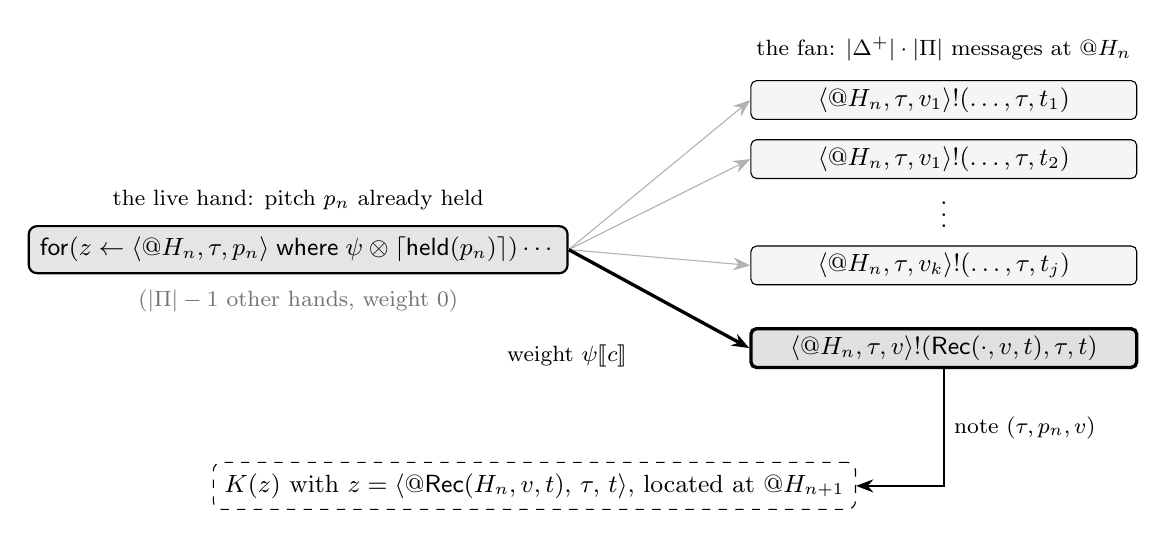
\begin{tikzpicture}[
  >={Stealth[length=2.2mm]}, font=\small,
  msg/.style={draw, rounded corners=2pt, inner sep=2.5pt, fill=black!4, minimum width=4.9cm},
  hand/.style={draw, thick, rounded corners=3pt, inner sep=4pt, fill=black!10}]
\node[hand] (h) at (0,0) {$\mathsf{for}(z \leftarrow \langle @H_n,\tau,p_n\rangle \;\mathsf{where}\;\psi\otimes\lceil\mathsf{held}(p_n)\rceil)\cdots$};
\node[font=\footnotesize, above=2pt of h] {the live hand: pitch $p_n$ already held};
\node[font=\footnotesize, below=2pt of h, text=black!55] {($|\Pit|-1$ other hands, weight $0$)};
\node[font=\footnotesize] at (8.2,2.55) {the fan: $|\Dur^+|\cdot|\Pit|$ messages at $@H_n$};
\node[msg] (m1) at (8.2,1.9)  {$\langle @H_n,\tau,v_1\rangle!(\ldots,\tau,t_1)$};
\node[msg] (m2) at (8.2,1.15) {$\langle @H_n,\tau,v_1\rangle!(\ldots,\tau,t_2)$};
\node      at (8.2,0.55) {$\vdots$};
\node[msg] (m4) at (8.2,-0.2) {$\langle @H_n,\tau,v_k\rangle!(\ldots,\tau,t_j)$};
\node[msg, very thick, fill=black!12] (mc) at (8.2,-1.25)
  {$\langle @H_n,\tau,v\rangle!(\Rec(\cdot,v,t),\tau,t)$};
\foreach \i in {1,2,4}{\draw[->, black!30] (h.east) -- (m\i.west);}
\draw[->, very thick] (h.east) -- (mc.west);
\node[font=\footnotesize, anchor=east] at (4.3,-1.35) {weight $\psi\llbracket c\rrbracket$};
\node[draw, dashed, rounded corners=3pt, inner sep=4pt] (nx) at (3.0,-3.0)
  {$K(z)$ with $z = \langle @\Rec(H_n,v,t),\,\tau,\,t\rangle$, located at $@H_{n+1}$};
\draw[->, thick] (mc.south) |- node[right, font=\footnotesize, pos=0.25]
  {note $(\tau, p_n, v)$} (nx.east);
\end{tikzpicture}
\caption{One step of a voice. The hands and the fan share the location $@H_n$,
the quote of the previous note's record. The fan is the same for every clause;
the clause weights its members and keeps exactly one hand live. The chosen
payload becomes the next location, so everything unchosen is left where no
receipt of this voice will be.}
\label{fig:voice}
\end{figure}

\subsection{Unbounded voices by reflection}\label{ssec:reflective}

The continuation $K$ must bring about the next step. It cannot contain it,
since that would make the term infinite; it asks for it. A per-voice
\emph{server} answers the request, and the server re-creates itself from its
own code, which it keeps on a code channel, re-sending the code each time it
reads it. Fix two bases $B_S$ and $B_C$ for the voice.
\[
\begin{array}{rcl}
\Req(z) &:=& \snd{\nm{B_S}{\tau}{\nulld}}{\drop z}{\tau}{\rest} \\[4pt]
\Server &:=& \rcv{w}{\nm{B_S}{\tau}{\rest}}{\big(\,\mathsf{Step}_{\Req}(w) \;\mid\; \Refresh\,\big)} \\[4pt]
\Refresh &:=& \rcv{c}{\nm{B_C}{\tau}{\rest}}{\big(\,\drop c \;\mid\; \snd{\nm{B_C}{\tau}{\nulld}}{\drop c}{\tau}{\rest}\,\big)} \\[6pt]
\Voice(p_0,u_0) &:=& \Server \;\mid\; \snd{\nm{B_C}{\tau}{\nulld}}{\Server}{\tau}{\rest}
  \;\mid\; \snd{\nm{B_S}{\tau}{\nulld}}{H_0}{\tau}{\rest}
\end{array}
\]

\noindent The server's text mentions only the fixed names built from $B_S$ and
$B_C$, the clause, and the alphabets. It does not mention itself: $\Refresh$
runs whatever code it finds, $\drop c$, and puts it back. So $\Voice$ is a finite
term, and nothing beyond Definition~\ref{def:syntax} is used.

\begin{proposition}[The machinery is silent]\label{prop:silent}
In every run of $\Voice(p_0,u_0)$:
\begin{enumerate}[label=(\roman*),itemsep=1pt]
\item the communications at $@B_S$ and $@B_C$ are null notes
  $(\tau,\rest,\nulld)$, and each musical note is followed by exactly two of
  them, a request and a refresh;
\item each has a single candidate, so it is resolved without chance and
  contends with nothing;
\item each has the onset of the musical note that follows it and adds no time,
  so the performance consists of the musical notes alone;
\item the voice is \emph{productive}: between two musical notes there are
  finitely many null notes.
\end{enumerate}
\end{proposition}
\begin{proof}
The request is a co-channel message of duration $\nulld$ at $@B_S$ and the
server listens there on a channel of pitch $\rest$; likewise at $@B_C$. At any
time $@B_S$ holds at most one server receipt and one request, since a request is
issued only by the live hand's continuation and the server is re-created only
after serving it; likewise $@B_C$ holds one refresh and one code message. The
request is stamped at the end of the note that issued it, so the server fires
at that time, adds $\len{\nulld} = 0$, and stamps the next step with the same
time; so does the refresh.
\end{proof}

\begin{remark}[Why a server, and why every hand]\label{rem:whyserver}
Two shortcuts fail, and they explain the shape. Code carried as a message's
payload cannot mention the name it will arrive on, because that name's location
is the quote of the payload itself, and a finite term cannot contain its own
quote. So the name must be handed to the code, which is what the request does.
And a name handed over by a message takes its datum from that message, which the
sender can only write literally; so the step cannot rebuild the hand holding
the recorded pitch, and instead offers a hand for every pitch and lets the
clause keep one live. Both costs are paid in null notes and inert receipts, and
neither is heard.
\end{remark}

\subsection{Freshness: the unplayed is inert}

Along a run write $H_{n+1} := \snd{\nm{H_n}{\tau}{\delta_n}}{H_n}{\tau}{p_{n+1}}$,
where $(p_n,\delta_n)$ is the $n$-th note and $p_{n+1}$ the pitch it carried.

\begin{lemma}[Freshness]\label{lem:fresh}
(i) Along one run the locations $@H_0, @H_1,\dots$ are pairwise inequivalent,
and inequivalent to the voice's bases. (ii) If two voices have inequivalent
bases, no location reached by one is equivalent to one reached by the other,
whatever choices are made.
\end{lemma}
\begin{proof}
Up to the unit law a record is a single message, and congruence identifies a
single message only with one whose subject and payload are congruent. So
$H_n \scong H'_m$ with $n \le m$ unwinds to $H_0 \scong H'_{m-n}$. If $m>n$ the
right side's payload is a record while $H_0$'s is a base, a receipt; if the
bases differ the unwinding ends on two inequivalent receipts. Bases are
receipts, records are messages.
\end{proof}

\begin{lemma}[The unplayed is inert]\label{lem:inert}
In every configuration reachable from a voice, among the record locations only
the current one, $@H_n$, holds a candidate of positive weight, and all of its
candidates belong to the live hand. The hands and messages left at earlier
locations never take part in a communication.
\end{lemma}
\begin{proof}
Each musical note consumes the live hand and one fan message at $@H_n$, and the
next step is placed at $@H_{n+1}$; by Lemma~\ref{lem:fresh} nothing is ever
placed at an earlier location. The other hands at $@H_n$ carry a crisp factor
that reads the fixed location and is false there.
\end{proof}

The leftovers are the continuations that were not played: inert, and a record
of what was chosen against. More importantly for what follows, \emph{the
location of a voice is its past}. $H_n$ contains every note the voice has
played, nested, the most recent outermost. A spatial formula under the name
predicate can therefore read the recent past to any finite depth, and this is
the basis of \S\ref{sec:idioms}.

The hand's continuation cannot depend on which message wins except through the
name it receives, so the fan cannot be tailored and must offer all of
$\Dur^+\times\Pit$; the transitions a clause forbids have weight $0$. The
process topology of a voice is the same for every clause: \emph{the musical
content is the clause}.

%==============================================================================
\section{Distributions}\label{sec:dist}

\subsection{The law of a voice}

For a candidate at $@H_n$ write $\pi = p_n$ for the held pitch, $\delta$ for its
duration, $\kappa$ for its carried pitch, and $h_n$ for the past recorded in
$H_n$.

\begin{theorem}[The law of a voice]\label{thm:law}
Let a voice run with clause $\psi$ and suppose that at each location some
candidate has positive weight. Conditionally on the past, the $n$-th fitting
emits $(p_n, v)$ and carries $t$ with probability
\[
\frac{\psi\llbracket (p_n, v, t, h_n)\rrbracket}
     {\sum_{v',t'} \psi\llbracket (p_n, v', t', h_n)\rrbracket} .
\]
\end{theorem}
\begin{proof}
Invariant: after $n$ musical notes and the null notes that follow them, the
configuration is congruent to
$\mathsf{Step}_{\Req}(\nm{H_n}{\tau}{\rest}) \mid \Server \mid C \mid G_n$, with
$C$ the code message and $G_n$ inert at earlier locations. By
Lemma~\ref{lem:inert} the only musical contention set is the star of the live
hand at $@H_n$, whose maximal matchings are single candidates, one per $(v,t)$;
the null notes are resolved without chance (Proposition~\ref{prop:silent}).
Apply Definition~\ref{def:resolve}. Firing passes
$z = \nm{\Rec(\nm{H_n}{\tau}{p_n},v,t)}{\tau}{t} \nameq \nm{H_{n+1}}{\tau}{t}$;
the request and refresh then re-establish the invariant at $n+1$, and the other
hands and fan messages join $G_{n+1}$.
\end{proof}

\begin{example}[Markov idioms]\label{ex:markov}
With weighted state machines $w_\Pit$ on pitches and $w_\Dur$ on durations,
\[
\psi_{M} :=
\Big(\bigoplus_{(s,t)} \crisp{\atm{pitch}(s)\wedge\atm{carry}(t)} \tensorv w_\Pit(s,t)\Big)
\tensorv
\Big(\bigoplus_{(u,v)} \crisp{\atm{prev}(u)\wedge\atm{dur}(v)} \tensorv w_\Dur(u,v)\Big),
\]
where $\atm{prev}(u) := \atm{at}(\langle{-},{-},u\rangle!\,\top)$ reads the last
duration from the location. By Theorem~\ref{thm:law} and the factorisation
below, the pitch and duration streams are independent Markov chains with the
row-normalised matrices. This is the simplest idiom; everything that follows
refines it.
\end{example}

\begin{remark}[The instrument as a score]\label{rem:skein}
F1R3Skein's streams are Example~\ref{ex:markov} with the player's drawn
machines, and its original digit streams are the uniform complete machines
resolved, factor by factor, by interval decoding of two constants
\cite{SkeinDrawn}. The simulator confirms that this reproduces the digit
streams exactly (Finding~\ref{find:embed}). It is one score among many.
\end{remark}

\subsection{Combining distributions}\label{ssec:combine}

A composer rarely wants one monolithic table. The clause algebra gives three
ways to combine preferences, and they have different meanings.

\paragraph{Product: all preferences at once.}
If $\psi = \psi_1 \tensorv \cdots \tensorv \psi_k$, a candidate's weight is the
product of its factors' weights, and by Theorem~\ref{thm:law} the played
distribution is the normalised pointwise product --- what the machine-learning
literature calls a product of experts. A continuation is likely only if every
factor finds it acceptable, and any factor can veto with a $0$.

\begin{lemma}[Factorised resolution]\label{lem:factor}
If a star's candidates are indexed by $A\times B$ and
$\psi\llbracket(a,b)\rrbracket = f(a)\,g(b)$, resolving the star is the same as
drawing $a \propto f$ and, independently, $b \propto g$.
\end{lemma}
\begin{proof}
The normalised product is the product of the normalisations.
\end{proof}

\noindent So factors that look at disjoint aspects --- pitch and duration, say
--- are heard independently, and may be realised by separate chance sources.
Factors that look at the same aspect interact: a style factor and a physicality
factor on the same pitch choice reweight each other.

\paragraph{Sum: a mixture of styles.}
$\psi_1 \sumv \psi_2$ adds weights. Where the two factors have comparable total
mass at a location, the result is close to a mixture that sometimes speaks one
idiom and sometimes the other; scaling one summand by a constant sets the
blend.

\paragraph{Convolution: intervals rather than pitches.}
A factor that depends only on the interval,
$\psi_I = \bigoplus_k \crisp{\atm{step}(k)} \tensorv w(k)$, makes the pitch
walk a sum of intervals. Away from the edges of the alphabet and with no other
pitch factor, the distribution of the pitch after $n$ fittings is the $n$-fold
convolution of the normalised interval law with the starting point; multiplying
two interval factors reweights the steps, and composing two voices' interval
laws in sequence convolves them. Most idioms are interval-shaped at least in
part, and this is where the word ``convolving'' is literal.

\subsection{Style}

A style, for the purposes of a score, is a factor --- or a small product of
factors --- over the choices a voice makes. The examples below are sketches of
the \emph{shape} such factors take, not claims to have captured the idioms.
\begin{itemize}[leftmargin=*,itemsep=2pt]
\item A rock-and-roll melodic factor might favour minor-pentatonic and blues
  degrees over a major harmony, with a duration factor favouring swung or
  straight eighths; swing needs a duration alphabet with triplet values, which
  the composer supplies.
\item A country melodic factor might favour major-pentatonic degrees and
  stepwise approach to chord tones, with a duration factor favouring even
  subdivisions.
\item Both can depend on the past through the location
  (\S\ref{sec:idioms}), so ``approach the chord tone from a semitone below'' is
  a factor over the last two pitches, not a table over one.
\end{itemize}
The point is architectural. Because the style is a factor, it can be held fixed
while the physicality changes, blended with another style by $\sumv$, or
hardened into a rule by replacing a small weight with $0$.

\subsection{Physicality}\label{ssec:physical}

Instruments make some continuations easy and others hard, and players follow
their hands. A \emph{physicality factor} weights candidates by that ease.

\paragraph{Melodic physicality.} For a single line, ease depends on the interval
and, often, on where the hand is. The interval part is an interval factor. The
position part needs the past: a fretted or bowed instrument's hand position is
a function of the last few notes, which the location records, so a factor under
$\atm{at}(\cdot)$ can prefer continuations near the current position. The
simulator measures the effect of exchanging such a factor under a fixed style:
a stepwise instrument and a leaping instrument give measurably different lines
from the same style factor (Finding~\ref{find:convolution}).

\paragraph{Vertical physicality, and why it needs coupling.} Closed-voice
stacked thirds lie naturally under a pianist's hand, while across adjacent
strings tuned in fifths they are awkward to impossible, and open voicings built
on fifths lie naturally instead. A preference of this kind relates
\emph{simultaneous} notes. Independent voices cannot express it: by
Theorem~\ref{thm:harmony} their choices are independent. That is correct
musically, since a hand is not a set of independent fingers, and it means that a
hand's vertical physicality must be written as a coupling. The graded join of
Paper~II supplies it.

\begin{definition}[Chords as joins]\label{def:join}
A \emph{chord receipt}
$\mathsf{for}(y_1 \leftarrow x_1 \,\&\, \cdots \,\&\, y_k \leftarrow x_k
\;\mathsf{where}\;\psi)P$, with $x_1,\dots,x_k$ channels at one location,
fires only when each pattern is matched by a distinct co-channel message at that
location. It emits the $k$ notes of its patterns at one onset, and its
continuation's receipts are stamped at the onset plus the longest of the $k$
durations. Its candidates are the injective assignments of messages to
patterns, and its clause sees all of them together: atoms
$\atm{pitch}_i, \atm{dur}_i, \atm{carry}_i$ for each pattern.
\end{definition}

A chord receipt is one receipt, so Proposition~\ref{prop:twosided} does not bite:
its contention set is a star and its alternatives are whole voicings. A piano
factor can then weight the voicing $(\kappa_1,\dots,\kappa_k)$ of the
\emph{next} chord by its span and by the intervals between adjacent chord tones,
favouring closed thirds within a hand's reach; a factor for strings tuned in
fifths can favour tones that fall on adjacent strings at the same stop. Every
other factor of the score is unaffected.

\paragraph{Imagined physicalities.} Nothing requires a physicality factor to
describe a human. A hand spanning three octaves, strings tuned in thirds, or a
factor that is uniform except for a vetoed interval are all one-line changes to
the score, and each gives the same style a new idiom.

%==============================================================================
\section{Motifs and idioms as formulae}\label{sec:idioms}

The grading says how strongly; the formulae say about what. They carry motifs
and idioms as much as the weights do.

\subsection{The past is readable}

Since the location is the past, the name predicate reads it. Define, over
pitch sequences $m$,
\[
\mathsf{Last}(\varepsilon) := \top ,
\qquad
\mathsf{Last}(m\cdot a) := \langle{-},{-},{-}\rangle!\big(\mathsf{Last}(m),\,{-},\,a\big),
\]
a formula of depth $|m|$ built from the output connective: the outermost record
carries $a$ and its payload satisfies $\mathsf{Last}(m)$. Then
$\atm{at}(\mathsf{Last}(m))$ holds exactly when the most recent pitches of the
voice, ending with the held pitch, are $m$. Durations are read the same way from
the records' subjects.

\begin{example}[Completing a motif]\label{ex:motif}
To encourage a voice that has played the head of a motif $m\cdot a$ to finish it
with $b$, multiply its clause by
\[
\big(\crisp{\atm{at}(\mathsf{Last}(m\cdot a))\wedge\atm{carry}(b)} \tensorv w\big)
\sumv 1 .
\]
Every candidate keeps its weight except the completion, which is multiplied by
$1+w$. Motif transformations are formulae relating the carried pitch to the
recorded ones: an answer transposed by $k$ is
$\crisp{\atm{at}(\mathsf{Last}(m\cdot a))\wedge\atm{carry}(a+k)}$, an inversion
negates the intervals, and so on.
\end{example}

\subsection{Enforcing an idiom}

A crisp factor is a rule. If $\beta$ is a crisp formula over the view of
Definition~\ref{def:cand}, then under $\psi\tensorv\crisp{\beta}$ no candidate
violating $\beta$ is ever played. Rules can conflict with the rest of the score,
and a voice with no positive candidate falls silent for good. A behavioural
modality prevents that.

\begin{proposition}[Enforcement without deadlock]\label{prop:enforce}
Let $\beta$ be a crisp condition on candidates, let $K$ range over the one-hole
contexts supplied by the rest of the score, and let
\[
\mathsf{Viable}_\beta \;:=\; \nu X.\;\bigvee_{K}\langle K\rangle_\beta\, X,
\]
where $\langle K\rangle_\beta X$ holds when some $\beta$-satisfying candidate
leads, in context $K$, to a configuration satisfying $X$. If the initial
configuration satisfies $\mathsf{Viable}_\beta$, then a voice with clause
$\psi\tensorv\crisp{\beta}\tensorv\crisp{\atm{leads}(\mathsf{Viable}_\beta)}$,
where $\atm{leads}(\gamma)$ holds of a candidate whose residue satisfies
$\gamma$, (i) never plays a note violating $\beta$ and (ii) never falls silent,
provided $\psi$ is positive on some $\beta$-satisfying candidate at every step.
\end{proposition}
\begin{proof}
(i) is immediate from the crisp factor. For (ii), $\mathsf{Viable}_\beta$ is a
post-fixed point: every configuration satisfying it has a $\beta$-candidate
whose residue satisfies it again. The clause admits exactly such candidates, so
viability is an invariant of every run, and an invariant configuration always
has a positive candidate.
\end{proof}

The greatest fixed point is in the ideal logic. It is decidable when $\beta$
reads a bounded window of the past and the pitch and duration alphabets are
finite, because the relevant state is then the window, the held pitch and the
recorded duration --- a finite graph on which $\nu$ is computed by iteration.
This is the ideal-versus-checkable-fragment discipline of the rho-life notes:
the ideal formula defines the idiom and the finite fragment decides it. The
context labels matter: an idiom such as ``a leading tone resolves up'' may be
viable alone and not in the company of a particular bass line, and
$\langle K\rangle$ is how the formula knows the company.

\subsection{Message passing as musical structure}\label{ssec:exchange}

Much of what is hard to notate is who plays in response to whom. Here that is
the communication structure of the score, and the formulae give the responder
access to what it is responding to.

\paragraph{Handoff: call and response, trading phrases.} A caller plays a
phrase and hands the line to a responder in the responder's timbre. Let $R$ be a
rendezvous location used once. A phrase has a written length $k$, so the caller
needs no server: it is $k$ steps written out, and the live hand of the last one
continues with $\Call(z)$ instead of a request. $\Call$ emits the fan at $R$
rather than at the caller's own location, addressed in the responder's timbre
$\tau_B$. The responder waits at $R$:
\begin{gather*}
\Call(x) \;:=\; \prod_{v,t}\;\snd{\nm{R}{\tau_B}{v}}{\Rec_B(x,v,t)}{\tau_B}{t},
\\
\Resp \;:=\; \rcvw{y}{\nm{R}{\tau_B}{p_B}}{\psi_B}{\Req_B(y)},
\end{gather*}
where $\Rec_B$ is $\Rec$ in timbre $\tau_B$, $p_B$ is the written first pitch
of the response, and $\Req_B$ asks the responder's own server for its next step.

\begin{proposition}[Handing over the history]\label{prop:handoff}
The responder's first note is $(\tau_B, p_B, v)$ for a fan message chosen by
$\psi_B$, and from then on the responder's location has the caller's entire
history as a sub-record. In particular $\psi_B$ can read the call: on the first
fitting through $\atm{passes}(\cdot)$, and afterwards through $\atm{at}(\cdot)$.
\end{proposition}
\begin{proof}
The payload of each $\Call$ message is $\Rec_B(x,v,t)$, whose payload is
$\drop x$, the caller's final location. The responder's continuation is placed
at the quote of that record. (The outermost record of the handoff also carries
the caller's last held pitch, which was never played; formulae reading the call
skip that one record.)
\end{proof}

With Example~\ref{ex:motif}'s transformation formulae, ``answer the call a fifth
higher'' or ``echo the call's rhythm with new pitches'' are clauses. Trading
phrases between several players is a chain of rendezvous, and because the
history is handed on, each player can respond to the whole exchange so far. In
this calculus the handoff is a note --- every communication is --- so passing
the line is itself musical: the responder's first note is where the line
changes hands.

\paragraph{Alternation: hocket and interlocking.} When two players share an
instrument's timbre, a single line can alternate between their clauses. Give
each player a server whose step uses that player's clause, and let each
player's live hand address its request to the \emph{other} player's server:
\begin{gather*}
\Server_A := \rcv{w}{\nm{B_{S_A}}{\tau}{\rest}}{\big(\mathsf{Step}^{\psi_A}_{\Req_B}(w) \mid \Refresh_A\big)},
\\
\Server_B := \rcv{w}{\nm{B_{S_B}}{\tau}{\rest}}{\big(\mathsf{Step}^{\psi_B}_{\Req_A}(w) \mid \Refresh_B\big)}.
\end{gather*}
The line is one line, so its interval and motif factors see every note, while
each player's clause adds that player's own preferences; the players' notes
interleave note for note. This is the shape of interlocking in which two parts
alternate strokes to form one resultant line, as with players sharing an
amadinda xylophone. Alternation between different timbres would need a
communication that changes timbre, which the rules do not yet allow.

\paragraph{Cross-rhythm: independence with a composer's alphabet.}

\begin{example}[Three against two]\label{ex:crossrhythm}
Let voice $A$ use only a triplet value of length $\tfrac{1}{6}$ and voice $B$
only a length of $\tfrac14$, both starting at $0$ from distinct bases. Their
onsets coincide exactly at multiples of $\tfrac12$, whatever pitches their
clauses choose, and by Theorem~\ref{thm:harmony} the pitch choices are
independent. Writing the rhythm as two independent processes, rather than as a
grid with a common subdivision, keeps each part's own pulse primary.
\end{example}

%==============================================================================
\section{Harmony}\label{sec:harmony}

\subsection{Independence gives free harmony}

\begin{theorem}[Harmony by independence]\label{thm:harmony}
Let two voices have any timbres and clauses, with pairwise inequivalent bases
(seed, server and code bases), and suppose neither clause mentions the other voice's
locations. Then (i) they are independent and every contention set belongs to
one voice; (ii) their joint law is the product of their laws; (iii) for fixed
choices every onset-ordered run has the same performance.
\end{theorem}
\begin{proof}
(i) Lemma~\ref{lem:fresh}(ii) and Lemma~\ref{lem:inert}; each voice's server
and code channel are at its own bases. (ii) Contention sets
are resolved with independent chance and each belongs to one voice. (iii)
Theorem~\ref{thm:interleave}.
\end{proof}

Nothing coordinates two such voices: each keeps its own clock in its own data,
and their notes do not depend on how their events interleave. When each voice
has its own chance source, (iii) holds surely.

\subsection{Coupling gives voicing}

\begin{proposition}[Simultaneity by contention]\label{prop:coupled}
Let two hands with distinct pitches and equal stamps share a location with a fan
of $n\ge2$ duration messages and a constant clause. One resolution emits two
notes at one onset whose durations are never equal, whereas independent uniform
draws coincide with probability $1/n$.
\end{proposition}
\begin{proof}
Proposition~\ref{prop:twosided} with $m=2$.
\end{proof}

Harmony between independent parts is free; voicing --- the relation between
simultaneous notes of one hand or one section --- is a coupling, written either
as shared locations or, with full control, as a chord receipt
(Definition~\ref{def:join}). The calculus keeps the two apart, and the composer
chooses which relation holds between which parts.

%==============================================================================
\section{Measurements}\label{sec:measured}

The reference simulator \texttt{skeinsim.py} is stdlib-only (it uses
\texttt{mpmath} only for the digits of $\pi$ and $e$ in one test). It
implements the calculus generically: quoted processes are hash-consed so that
location equivalence is identity; candidates come from the premises of the
communication rules; clauses are evaluated as formulae over the atoms, including
spatial atoms that walk the recorded past; and contention sets, maximal
matchings and onset ordering follow the definitions. The resolver knows nothing
of voices or idioms. Unless stated otherwise, machines are random over a
sixteen-pitch alphabet and five durations.

\begin{finding}[The unplayed is inert]\label{find:inert}
One voice, $400$ notes, collection off: at every step exactly one location holds
both a receipt and a message; $31{,}600$ messages, exactly $79 = 5\cdot16-1$ per
note, remain at earlier locations and none ever joins a candidate.
\end{finding}

\begin{finding}[The law of a voice]\label{find:law}
One voice with Example~\ref{ex:markov}'s clause, $20{,}000$ notes: over the
$54$ stochastic cells the largest deviation from the pitch matrix is $0.031$
($|z|\le 2.34$) and from the duration matrix $0.009$ ($|z|\le1.21$), with no
off-machine transition; over $117$ cells of the joint law of the two choices in
one fitting, the largest deviation from the product is $0.030$ ($|z|\le2.87$).
The rhythm-leads mirror image using $\textsc{Comm}_2$ gives $0.052$
($|z|\le2.25$) and $0.010$ ($|z|\le1.47$). All consistent with sampling error.
\end{finding}

\begin{finding}[Recursion by reflection is silent]\label{find:reflective}
The reflective voice of \S\ref{ssec:reflective}, run against a reference
implementation of the step semantics that writes the recursion in the
metalanguage, with the same clause and the same chance source for musical
choices: over $3{,}000$ notes the two performances are identical, note for note
and onset for onset. The reflective voice played $6{,}000$ null notes, exactly
two per note, every one a rest of length zero. Without collection, over $200$
notes, at most one record location ever held a candidate (at most two locations
counting the server and code channels, which fire concurrently with the next
note), and exactly $15 = |\Pit|-1$ inert hands were left behind per note.
\end{finding}

\begin{finding}[Product of style and physicality]\label{find:convolution}
A fixed random style factor over twenty-one pitches (four to seven
continuations each), multiplied in turn by two interval factors: a
\emph{stepwise} instrument weighting steps of at most two degrees $3$ and all
else $0.3$, and a \emph{leaping} one weighting intervals of four or seven
degrees $3$ and all else $0.3$. Over $20{,}000$ notes each, the empirical
transitions match the normalised product (largest $|z|$ $2.34$ and $2.76$) and
no transition the product forbids occurs. The same style played on the two
instruments: steps of at most two degrees are $0.582$ of intervals against
$0.135$; leaps of four or seven are $0.051$ against $0.378$; the mean interval
is $4.91$ against $6.97$ degrees.
\end{finding}

\begin{finding}[Idioms read from the past]\label{find:idioms}
One voice, $10{,}000$ notes per condition, with spatial atoms that walk the
recorded past. Unconstrained, the line contains $1{,}303$ three-fold repeated
pitches. With the crisp factor forbidding a pitch equal to the last two, it
contains none, and the voice never falls silent. With the motif-completion
factor of Example~\ref{ex:motif} ($w = 20$) for the motif $0,2,4$, the rate at
which the head $0,2$ is completed by $4$ rises from $0.171$ to $0.775$, against
analytic values of $0.154$ and $0.792$.
\end{finding}

\begin{finding}[Two-sided fitting]\label{find:twosided}
Three pitch receipts and four duration messages at one location, $2{,}000$
trials: under maximal matchings the first resolution emits $3.0$ notes and
nothing remains; one at a time, the first emits $1.0$ and the leftovers $2.0$
more, exactly as Proposition~\ref{prop:twosided} states.
\end{finding}

\begin{finding}[Harmony and coupling]\label{find:harmony}
Two voices on distinct bases, each with its own random stream, $3{,}000$
resolutions under five schedulers (either voice first on ties, three random
tie-breaks): the five performances are identical, with $216$ simultaneous
strikes. Two hands sharing a location with five duration messages, $20{,}000$
trials: every resolution emits two notes and their durations are never equal
(independent draws would coincide with probability $0.2$).
\end{finding}

\begin{finding}[The instrument as a score]\label{find:embed}
Uniform complete machines resolved by interval decoding, pitch from the
hexadecimal digits of $\pi$ and duration from the base-$5$ digits of $e$: for
$400$ notes the streams equal the digit streams and each draw consumes exactly
one digit.
\end{finding}

%==============================================================================
\section{Open threads}\label{sec:open}

\begin{enumerate}[leftmargin=*,itemsep=3pt]
\item \textbf{Tempo.} Time is already in the data (Remark~\ref{rem:time}), so
  tempo can enter as a second clause, valued in a second resolution algebra,
  scaling $\len{\delta}$ when a continuation is stamped: rubato per voice, a
  shared tempo over a shared namespace.
\item \textbf{A surface syntax for composers.} The calculus is a core. A
  composer needs named factors, a library of styles and physicalities, and
  a way to write phrases literally where nothing should be drawn.
\item \textbf{Learning styles.} Paper~II's gradient in the fibre applies
  directly: the weights of a style factor can be fitted to a corpus, and the
  formulae chosen by the composer say which features the learner may use.
\item \textbf{Timbre change.} Alternation across different timbres, and
  orchestration generally, need a communication whose payload timbre may differ
  from its subject's.
\item \textbf{Joins in full.} Definition~\ref{def:join} fixes one convention for
  when a chord's continuation starts; others (earliest release, per-voice
  continuations) give different idioms and deserve comparison.
\item \textbf{Productivity in general.} A voice plays two null notes per
  musical note (Proposition~\ref{prop:silent}). An arbitrary score can loop
  through null notes forever at one instant. A syntactic check that every cycle
  of null notes passes through a note of positive length would rule this out;
  it is not given here.
\item \textbf{Complex grading.} Over $\Cx$, two melodic paths to the same
  configuration would interfere. A voice already has what Paper~I's quantum
  fragment needs --- a single linear hand and locations that never repeat ---
  so audible interference between phrasings is a live question.
\end{enumerate}

%==============================================================================
\begin{thebibliography}{99}

\bibitem{GWpln}
L.~G.~Meredith. Graded where-clauses over the reals. F1R3FLY.io working note,
2026. Paper~II of three.

\bibitem{GWquantum}
L.~G.~Meredith. Races decided by the Born rule. F1R3FLY.io working note, 2026.
Paper~I of three.

\bibitem{Omnibus}
L.~G.~Meredith. Observation disciplines: how logics are generated from term
structure. F1R3FLY.io omnibus, 2026.

\bibitem{WeightedGSLT}
L.~G.~Meredith. Weighted graph-structured lambda theories. F1R3FLY.io working
note, second version, 2026.

\bibitem{SkeinSpec}
F1R3FLY.io. F1R3Skein instrument specification, revision 4.
\texttt{publications/f1r3skein}, 2026.

\bibitem{SkeinDrawn}
F1R3FLY.io. F1R3Skein: drawn distributions, revision 1.
\texttt{publications/f1r3skein}, 19 September 2026.

\bibitem{Mer05}
L.~G.~Meredith, M.~Radestock. A reflective higher-order calculus.
\emph{Electronic Notes in Theoretical Computer Science} 141(5):49--67, 2005.

\bibitem{NSL}
L.~G.~Meredith, M.~Radestock. Namespace logic: a logic for a reflective
higher-order calculus. \emph{Trustworthy Global Computing}, LNCS 3705, 2005.

\bibitem{CairesCardelli}
L.~Caires, L.~Cardelli. A spatial logic for concurrency.
\emph{Information and Computation} 186(2):194--235, 2003.

\bibitem{Gillespie}
D.~T.~Gillespie. Exact stochastic simulation of coupled chemical reactions.
\emph{Journal of Physical Chemistry} 81(25):2340--2361, 1977.

\end{thebibliography}

\end{document}
